\section{Architecture for Embedded Software Verification}
\label{architecture_s}	
Figure~\ref{architecture} presents the overall proposed architecture for ensuring Java bytecode correctness. 
\begin{figure}[ht!]
\begin{center}
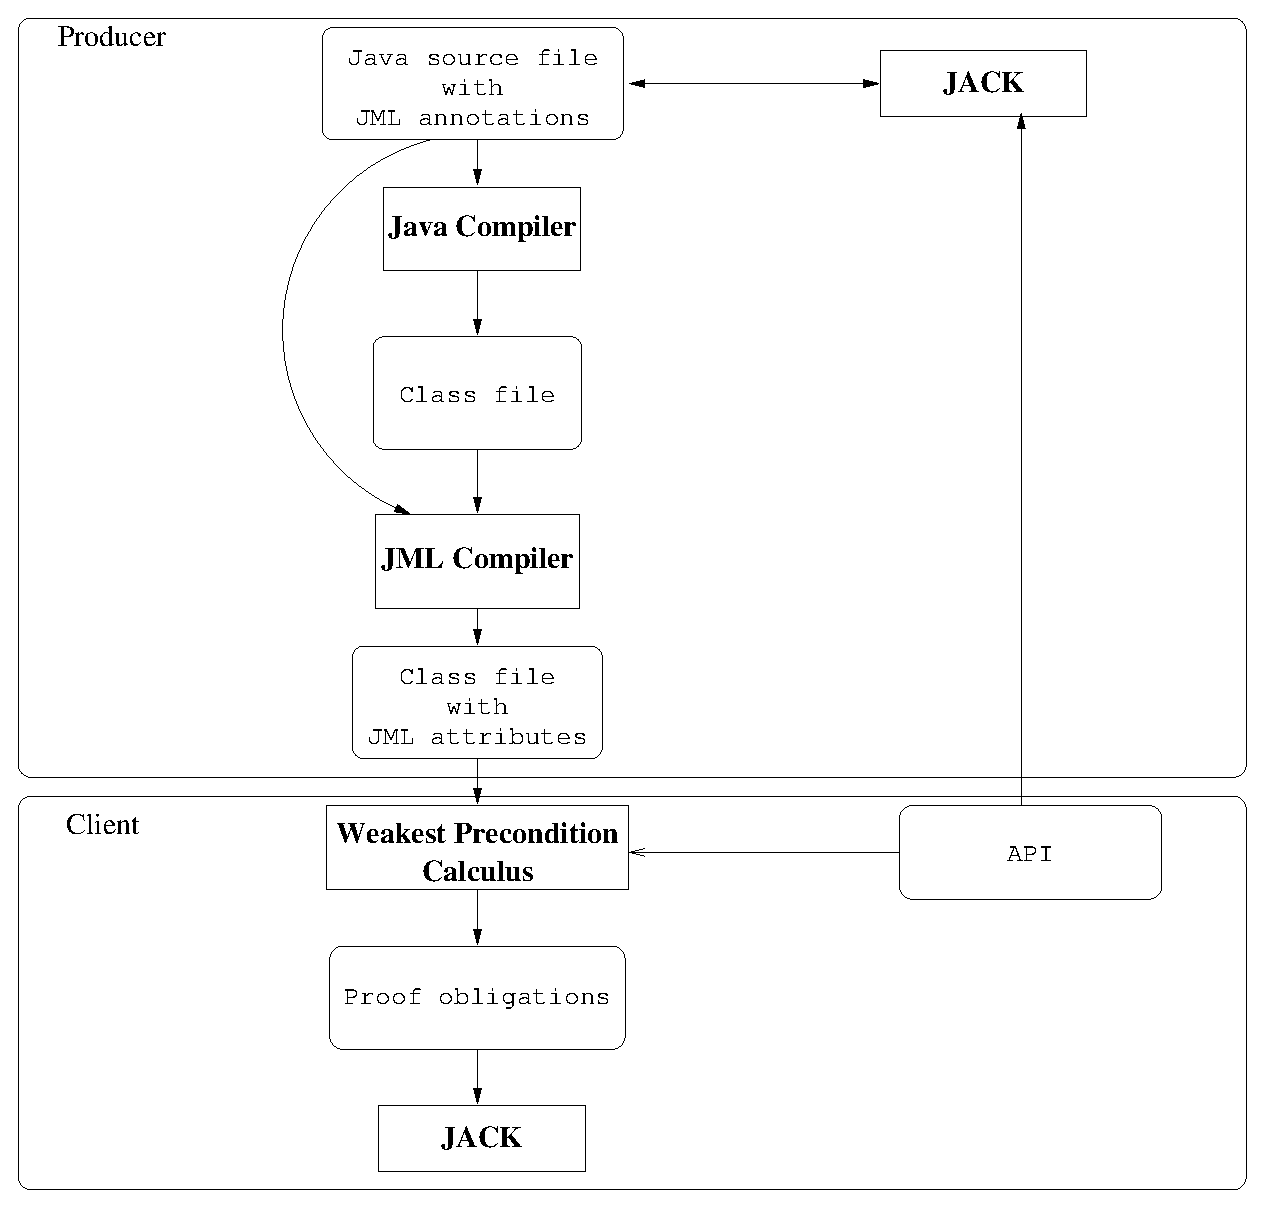
\epsfig{file=architecture.eps, width=\linewidth}
\caption{The overall architecture of the annotating and verifying code}
\label{architecture}
\end{center}
\end{figure}
It describes a process that allows a client to trust a code produced by an unstruted code producer.

The process starts with some annotated Java source files provided by a client to a code producer. Those files can be
\begin{itemize}
\item A specified interface that described the application that should be developped. In these case, the client can fully specified in JML the features that have to be implemented by the code producer.
\item An API with some restricted access to some method. In these case, the client can protect its system by restrecting its usage (for example: ...). 
\end{itemize}
In both cases, the code producer develops its application and proves that it fullfills the given requirements using Jack; 
in most cases, to complete this task, some annotations have to be added to the code.
When the annotations are sufficient to prove the code, the Java file is then normally compiled with a Java compiler to obtain a 
class file. 
This class file is then annotated with special JML attributes extracted from the source file. 
At this stage, the Java class files contain all the informations that will allow the client to trust it.

So the code can reach the client side where proof obligations are generated (at code level) with respect to client's requirements. 
The corresponding proof obligations are then proved, for instance, with the JACK framework. If the client succeeds in proving 
the verification conditions, he can trust the unknown code. 
%As is shown on the figure~\ref{architecture} in the general case we do not specify who does the proof. It may be the client, 
%the code producer or a third party. Here in this paper we consider that it is the client that genrates the proof.

In this framework, it is not necessary for the client to have an access to the source to verify high level properties. 
Nevertheless those properties can be expressed easily at source level.

To implement this framework, we have defined an extension of the class file format, we have implemented a tool to insert 
those special attributes in the class file and we have extended the Jack framework to generate proof obligations at bytecode level and to prove them with the plugged Jack provers. The next sections introduce those features.  

